% Time-stamp: <09/10/02 01:57:13 vilhuber>
% $Id: Presentation-PSD.tex 3219 2012-09-27 07:47:11Z vilhu001 $

% normal line:
\documentclass[xcolor=table,compress]{beamer}
% to create notes:
%\documentclass[handout,notes=only]{beamer}
% to create handouts
%\documentclass[xcolor=table,handout,compress]{beamer}
% to create a different kind of handouts
%\documentclass{article}
%\usepackage[envcountsect]{beamerarticle}

%\setbeameroption{handout}
%\setbeameroption{show notes}


%
% Packages
%
\mode<article> % only for the article version
{
  \usepackage{fullpage}
  \usepackage{hyperref}
}
\usepackage{ifpdf}
\ifpdf
\usepackage{embedfile}
\embedfile{\jobname.tex}
\fi

\usepackage{graphicx}
%\usepackage{pstricks}
\usepackage{xcolor}
\usepackage{pifont}
%\usepackage{../chicago}
\usepackage{pgf}
\usepackage{amsmath,amssymb,amsfonts}
\usepackage[latin1]{inputenc}
\usepackage{colortbl}
\usepackage[english]{babel}
\usepackage{array}
\usepackage{pdfpages}
% usage:
%   \includepdf[pages={1}]{myfile.pdf}
%   \includepdf[pages={1,3,5}]{myfile.pdf} would include pages 1, 3, and 5 of the file. 
%   To include the entire file, you specify pages={-}, where {-}
%\usepackage{landscape}
\usepackage{listings}
\lstloadlanguages{R,bash}
\lstset{numbers=left, stepnumber=1,  language=bash, basicstyle=\tiny}

%\usepackage{lmodern}
%\usepackage[T1]{fontenc}

\usepackage{times}
%\usepackage{colortbl}

%============================================================
% Beamer specific styles and configs
%============================================================

\mode<presentation>
{
% alternative, could always use
%\usetheme{Census}
\usetheme{cornell}
\useoutertheme{cornell}
}


%\setbeamercovered{dynamic}



%============================================================
% Title
%============================================================

\title[Computing for Economists]{Workshop: High-performance computing for economists}
\author[Vilhuber, Abowd, Mansfield, McKinney]{%
  Lars~Vilhuber\inst{1} \and
  John M. Abowd\inst{1} \and
  Richard~Mansfield\inst{1} \and
  Kevin~L.~McKinney %\inst{2}%
}

\institute[Cornell]{
  \inst{1}%
   Cornell University, Economics Department,
%\and \inst{2} U.S. Census Bureau
}%
\date[August 20-22, 2013]{August 20-22, 2013: Day 3}
\subject{HPC}


% % % % % % % % % % % % % % % % % Main document
\begin{document}
\frame{\titlepage}
\section{What is HPC?}

\begin{frame}{Discussion of HPC}
\href{http://www.vrdc.cornell.edu/computing-for-economists/documents/XSEDE_ICE_2012.pdf}{XSEDE
 presentation by Phil Blood, PSC (2012)}
\end{frame}

\section[HPC resources]{HPC resources at Cornell and elsewhere}

\begin{frame}{ECCO}
\href{http://www2.vrdc.cornell.edu/ecco/}{http://www.vrdc.cornell.edu/ecco/}
\end{frame}

\begin{frame}{Clusters}
\begin{block}{What are clusters?}
\begin{itemize}
\item \href{http://www.rocksclusters.org/wordpress/}{http://www.rocksclusters.org/}
\item \href{http://www.clusterresources.com/torquedocs21/2.1jobsubmission.shtml}{Torque Job Submission}
\item \href{http://star.mit.edu/cluster/docs/latest/index.html}{STAR Cluster}
\item \href{http://www.oracle.com/us/products/tools/oracle-grid-engine-075549.html}{Oracle (Sun) Grid Engine}
\end{itemize}
\end{block}

\end{frame}

\begin{frame}{Where are clusters?}
\begin{itemize}
\item \href{http://www.cac.cornell.edu/services/hpcsystems.aspx}{CAC Private Clusters} [Rocks]
\item \href{https://www.xsede.org/}{XSEDE}
\end{itemize}
\end{frame}


\begin{frame}{Where can I get computers?}
\begin{itemize}
\item Buy them (Dell, etc.)
\item Buy a subscription: \href{http://www.cac.cornell.edu/RedCloud/}{CAC RedCloud} [\href{http://www.eucalyptus.com/}{Eucalyptus}]
\item Rent them: \href{http://docs.aws.amazon.com/AWSEC2/latest/UserGuide/using-spot-instances-cluster.html}{Amazon EC2} (\href{http://star.mit.edu/cluster/docs/latest/quickstart.html}{STAR cluster})
\item Steal them: \href{http://en.wikipedia.org/wiki/Srizbi_botnet}{Botnet with 450,000 computers}
\item Use free ones: \href{http://en.wikipedia.org/wiki/CPU_scavenging}{CPU scavenging} \newline(\href{http://en.wikipedia.org/wiki/HTCondor}{HTCondorG}, \href{http://setiathome.berkeley.edu/}{SETI@Home})
\end{itemize}
\end{frame}

\begin{frame}{Getting access}
\begin{block}{...legally}
\begin{itemize}
\item \href{http://www2.vrdc.cornell.edu/news/ecco/step-1-requesting-an-ecco-account/}{Apply for an account on ECCO}
\item Accounts on CAC general cluster no longer available
\item Buy resources at Amazon 
\begin{itemize}
\item 750 hrs/month free for the first year if using Micro instances
\item 0.615GB	, Very Low network performance
\end{itemize}
\item \href{https://www.xsede.org/using-xsede\#step3}{Apply for an XSEDE account}
\end{itemize}
\end{block}
\end{frame}

\subsection{Getting access to a compute cluster}

\begin{frame}
\begin{block}{Linux}
\begin{itemize}
\item used on most compute clusters
\item used on very few desktop computers
\item but...
\end{itemize}
\end{block}
\pause
\begin{block}{Bash}
\begin{itemize}
\item bash is a ``shell'' - a text interface command interpreter
\item bash or ksh (Korn shell) or csh (C-shell) are the most common
\item bash is available on Linux and \pause OSX
\item you can also download Cygwin, getting bash for Windows
\end{itemize}
\end{block}
\end{frame}

\begin{frame}{Access to your local compute cluster}
\begin{block}{Several on-campus compute resources}
\begin{itemize}[<+->]
\item Cornell Center for Advanced Computing (\href{http://www.cac.cornell.edu}{CAC})\newline 
\uncover<3->{\alert{$\rightarrow$ Thursday}}
\item Cornell Institute for Social and Economic Research 
(\href{http://www.ciser.cornell.edu}{CISER})\uncover<3->{\alert{$\rightarrow$ Thursday}}
\pause
\item Economics Compute Cluster Organization (ECCO), aka Social Science Gateway (SSG)
\end{itemize}
\end{block}
\end{frame}


\begin{frame}{Getting access to ECCO}
\begin{block}{You already have...}
\begin{itemize}
\item You have an account by virtue of participating in this class
\item Moving forward, you will be eligible to faculty-sponsored accounts
\item Currently soft-monitoring of resource usage
\end{itemize}
\end{block}
\pause
\begin{block}{... but do you have \textbf{access}?}
Have you logged in via SSH to reset your password? \newline \uncover<3->{\alert{$\rightarrow$ 
\href{http://www2.vrdc.cornell.edu/news/ecco/step-2-first-login/}{Instructions}}}
\end{block}
\end{frame}


\begin{frame}{Quick walkthrough, using Chrome SSH}
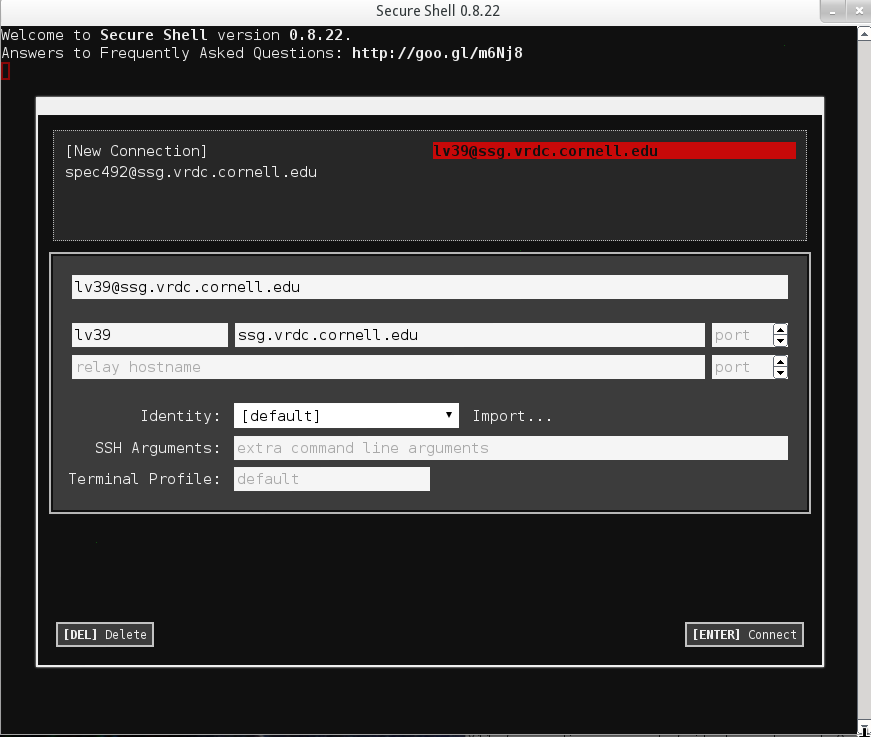
\includegraphics[width=.9\textwidth]{chrome-ssh-screen1.png}
\end{frame}


\begin{frame}{Quick walkthrough, using Chrome SSH}
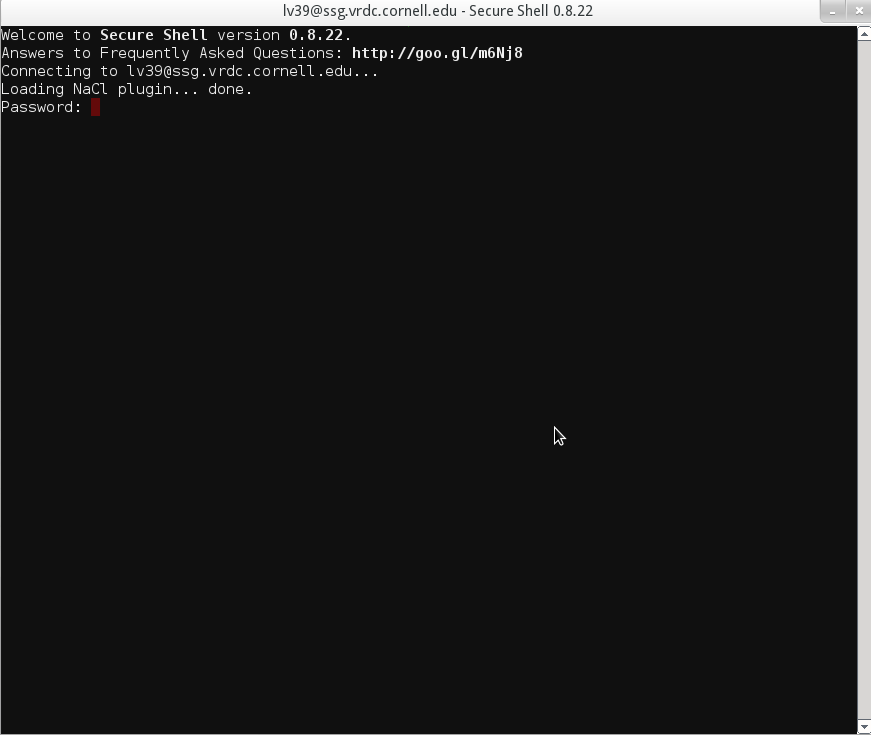
\includegraphics[width=.9\textwidth]{chrome-ssh-screen2.png}
\end{frame}


\begin{frame}{Quick walkthrough, using Chrome SSH}
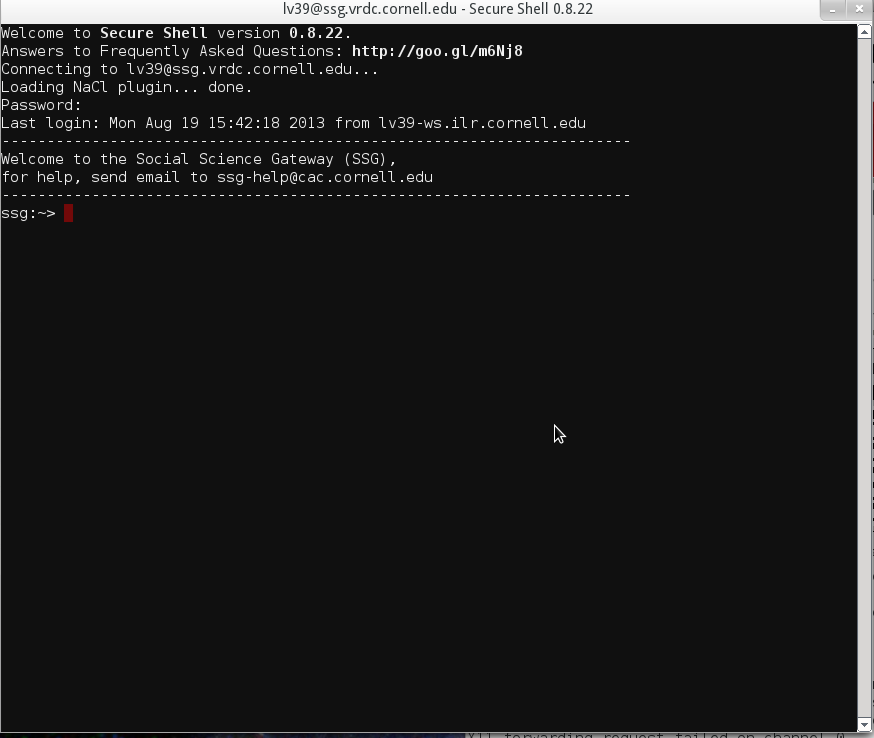
\includegraphics[width=.9\textwidth]{chrome-ssh-screen3.png}
\end{frame}



\begin{frame}{Access via NX}
\begin{block}{What is NX?}
NX is software similar to Windows Remote Desktop, allowing for a graphical interface to be made 
available remotely.
\end{block}
\begin{itemize}
\item Client is free (provided by Nomachine)
%\item We use a free server (not provided by Nomachine, but fully functional)
\item Clients can be launched by installing dedicated client (all OS)  
%or by launching the  webclient (currently not working for some Linux)
\end{itemize}
\end{frame}


\begin{frame}{Important note}
\begin{block}{NX on ECCO security}
You MUST download the custom-configured session from the VRDC website; the default session 
configuration from the NX client install will not work.
\end{block}
\tiny Details: we use a custom SSH key for the NX client, for some minimal additional security.
\end{frame}


\begin{frame}{Important note}
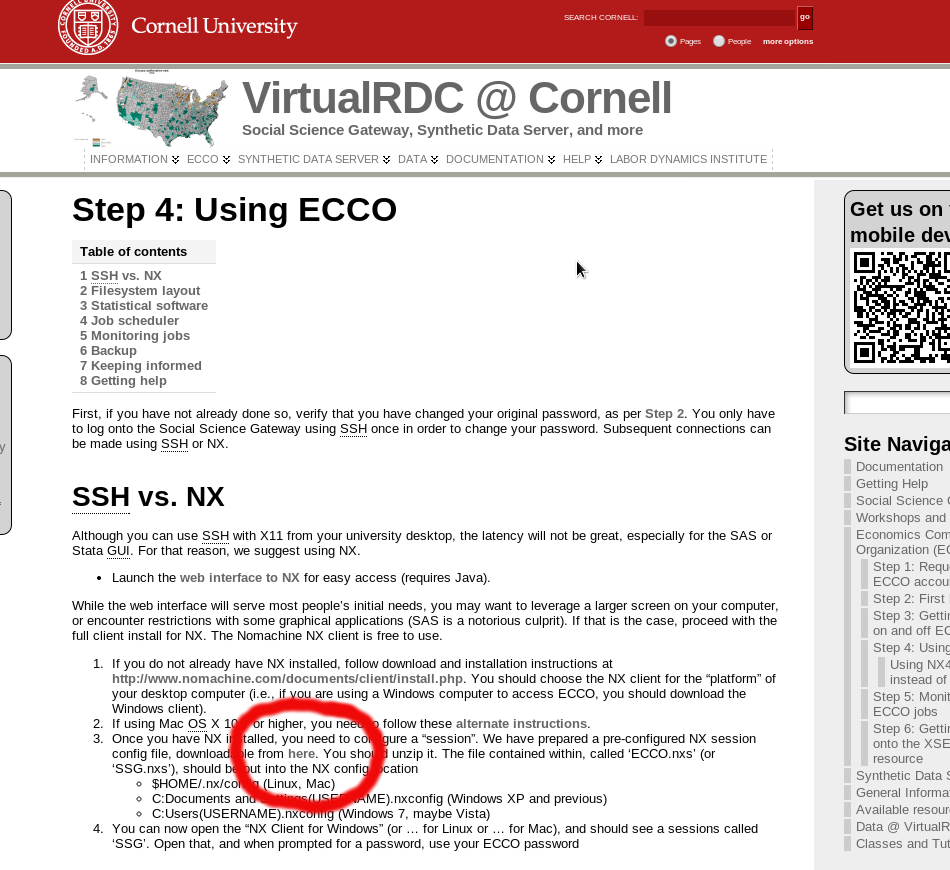
\includegraphics[height=.7\textheight]{nx-ecco-key.png}
\end{frame}


\begin{frame}{Logging on}
\centering
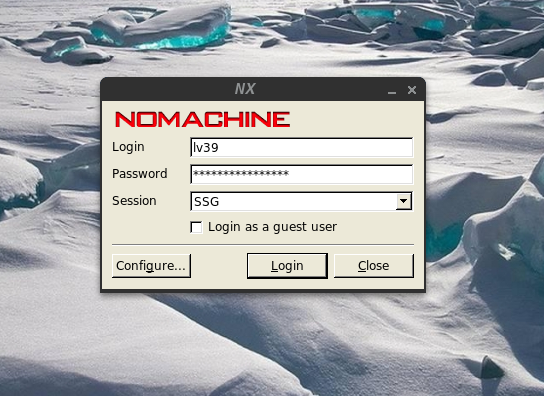
\includegraphics[height=.7\textheight]{nx-login-box.png}
\end{frame}


\begin{frame}{Successful connection}
\centering
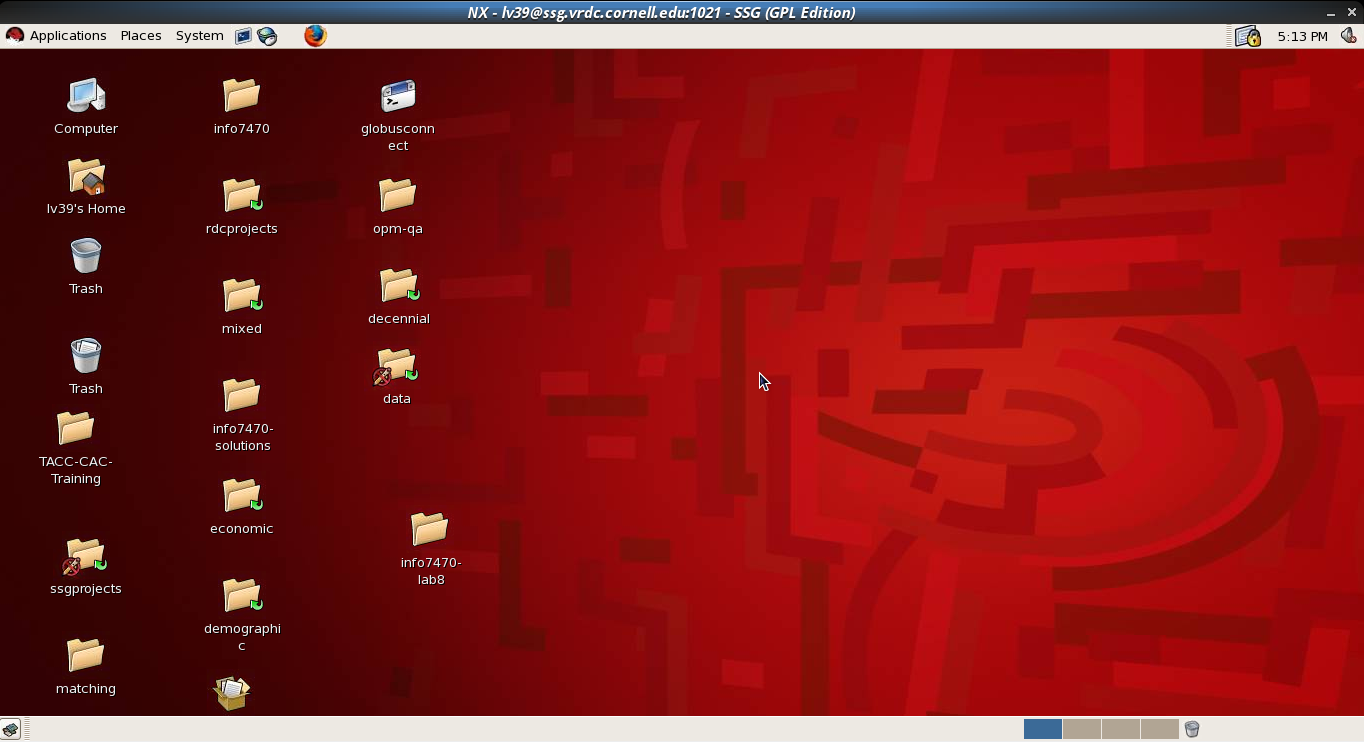
\includegraphics[width=1\textheight]{nx-logged-on.png}
\end{frame}


%\section[Data mgmt]{Considerations for data management}
%\begin{frame}
%\href{day3-2.pdf}{Data management}
%\end{frame}
%\section[Basics]{Basics of High-performance computing}
%\begin{frame}
%\href{day3-3.pdf}{Basics}
%\end{frame}
%
%
%\section{Wrap up}
%
%\begin{frame}
%\href{day3-4.pdf}{Wrap-up}
%\end{frame}

\end{document}